\section{The Git structure}
\emph{Git}, as it was said before, is a distributed version control system.
It means that each user has a mirror of the repository (local
repository) and in the case of
\emph{git}, there is no need for a central server, even if, each user is able to
fetch or push updates from other user's repository (remote repository).
\emph{Git} is divided mainly in three components. The working directory,
the index and the repository. The connection between these components
can be seen in Figure \ref{fig:git_structure}. Local and remote
repository have the same internal structure. What is a local
repository for an user is a remote repository for another user.

\begin{figure}[!t]
   \centering
   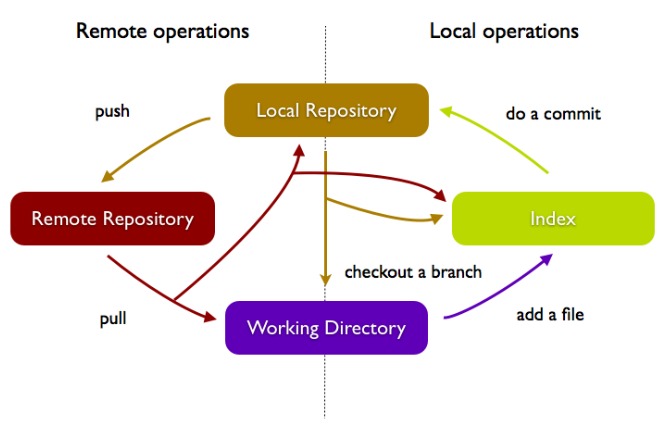
\includegraphics[width=0.8\textwidth]{images/git_workflow.png}
   \caption{Git WorkFlow}\label{fig:git_structure}
\end{figure}

\pagebreak

\section{The Repository}
\emph{Git} repository is like a database of a project along construction time. It is
the place where the snapshots taken during the project construction
are kept, as well as, all the necessary information to
allow the users to go through all the snapshots. The snapshot's
structure and snapshots' relations are kept using, what is called, \emph{git
objects}. The information needed to go through the project is kept in,
what is called, \emph{git references}. In the next subsections we
present both of them.


\subsection{Git Objects}
As we have presented before \emph{git} keeps snapshots of how your system
looked like on a certain moment in time. This moment in time is
represented in \emph{git} by a commit. Each commit points to a tree
(corresponding to a directory), that
represents the structure of your project on that moment. So a tree
contains others trees and/or blobs. In \emph{git} the files are not kept. 
What \emph{git} keeps is a object called blob that represents the content of files. The
relation between the path of a file and the content of that path 
is kept on the trees corresponding to that path. \par
In Figure \ref{fig:snapshot} is possible to see an example of a snapshot. We
have a commit that points to a tree. This first tree corresponds to
the root directory of the project. All the other trees (and blobs)
corresponds to some directory (or file) preserving the relation
between them. \par
In the next sections a detailed description about each object is
given, but for now something that is useful to know is that each
object is identified by a 40-character string. This string is
calculated by taking the SHA I hash of the contents of the object.
This approach has many advantages, being the two more important, in our
opinion, the
fact that it is possible to compare two objects only by the name and
if two objects have the same content then, only one of them is kept.\par

\begin{figure}[!h]
   \centering
   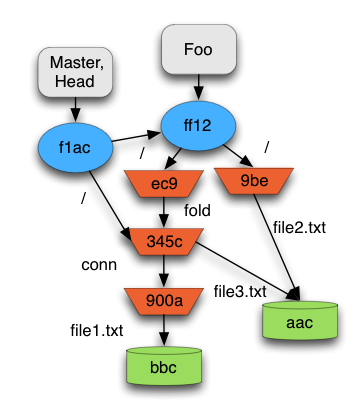
\includegraphics[width=0.4\textwidth]{images/object_assoc.png}
   \caption{A Snapshot}
   \label{fig:snapshot}
\end{figure}

\subsubsection{Blob}
A blob object, as it was said before, represents the content of a
file and the blob name is calculated from the blob content. So if we
have two files exactly with the same content, only one blob will be
kept, even if, they have different names . This happens because the
blob is not directly associated to a file. The relation between a path
(of a file) and a blob is kept in the tree object. 

\subsubsection{Tree}
A tree is nothing else than a map from names to blobs and other trees. This map
represents the contains relation. Also here, a tree is not associated to any 
specific directory.
If two directories have exactly the same content they will be
represented by the same tree object. Here have the same content means
that it should have exactly the same relations, or in other words, we
have exactly the same names in both trees and each name corresponds exactly
to the same objects in both trees. 

\subsubsection{Commit}
The commit object, is like a snapshot of the project on a certain moment in
time. A commit object has more variety of information than the two
objects addressed before. Looking a commit, it is possible to find out
the following:
\begin{itemize}
   \item Author - The person responsible for the change on the
   project.
   \item Committer - The person which actually created the commit. It
   is possible that the committer is different from the author. An
   author can create a patch, send it to the committer,
   which will create the commit.
   \item Parent - The previous commit, or, the commit from which this
   one was created. It is possible for this field to be empty, when 
   the commit is a Root Commit (the first commit to be done). 
   It is also possible to have two parents, when the commit is a result
   from a merge operation.
   \item Comment - It is possible, when creating a commit, write a
   comment about the commit. This comments can contain details about
   the changes that were done in the project, as well as, something
   that the Committer wants to write.
   \item Tree - It is a pointer for a tree, or in other words, it is a pointer
   for how the project looked like on a certain moment in time. 
\end{itemize}

In our model, we concentrated our efforts in the Parent and in the
Tree fields. We just care about the structure of the object model, so,
we removed everything else that does not influences such
structure. One property that we observed when modeling, is that, we
cannot have cycles in the parent relation. It means that if we are
on commit C1 and we go through the parent relation, we will never
reach C1.

\subsubsection{Tag}
At last we have the tag object. The tag object is just a pointer to
a commit with some more information. It can be used to mark a special 
commit, like a new version of the project. The structure is quite 
similar to the commit object. It has a tagger (the person who created 
the tag), a date in which the tag was created, a message (some
comment from the tagger) and it points to a commit object. In our
model we did not model this object, because when abstracting it looks
like a branch, that we will see in next section.

\subsection{Git References}
Basically a reference is just a pointer to a commit. There is much
more about references, but in this manual, lets keep it simple and
concentrate on the object model. In this manual, we just speak about
Branches and the special reference HEAD.

\subsubsection{Branches}
One of the trump cards of \emph{Git} is its definition of branches. In other
VCS each time a branch is created a new copy of the entire repository
has to be done. Thus, branches operations in those VCS are slow and hard to use. 
In \emph{git}, when a new branch is created the only thing that
\emph{git} does, is to create a new pointer to the current
commit. The current commit is marked by a special reference called
HEAD, that we present next.

\subsubsection{HEAD}
HEAD is maybe the most important reference in the repository. It
indicates where you are situated in the repository. When a commit is
done, \emph{git} has to know which commit is going to be the parent. 
It does so, looking into the HEAD. HEAD normally is a
pointer to a branch, so when the commit is done, the HEAD is kept, but
the branch points to the new commit. HEAD can point directly to a
commit, but lets keep it simple.

\section{Working Directory}

The working directory is basically a subset of
a file system that contains the files of the project you are
currently working on. These files can be the current files, files
retrieved from an old snapshot or even files that are not being
tracked. When retrieving an older snapshot of the project, the
working directory is updated to reflect the project in that state. The
untracked files in the working directory are just ignored, unless
there is a conflict when retrieving files from an older snapshot.\\

When a user starts a repository, all the files are untracked. When a
new file is created it will be untracked. So, how does \emph{git} know which
files are tracked or not? There exists the index which we present
next.

\section{Index}
The index is something in between the working directory and the
repository. When a file is created if the user wants that file to be
on the next commit, it has to be on index. Even if the user just
modifies a file and the user wants that change to be reflected on the
next commit, it must be added to index, otherwise, what will be
committed is the older version of the file. So, basically the index
contains all the files that will be in the next commit.\\

